%% Wosc6 Submission
\documentclass[sigplan, screen]{acmart}
\usepackage[utf8]{inputenc}
\usepackage{graphicx}
\usepackage{pgfplots}
\usepackage{listings}
\usepackage{color}
\usepackage{listings}
\usepackage{xcolor}
\usepackage{fancyhdr}


\definecolor{codegreen}{rgb}{0,0.6,0}
\definecolor{codegray}{rgb}{0.5,0.5,0.5}
\definecolor{codepurple}{rgb}{0.58,0,0.82}
\definecolor{backcolour}{rgb}{0.95,0.95,0.92}

\lstdefinestyle{mystyle}{
    backgroundcolor=\color{backcolour},
    commentstyle=\color{codegreen},
    keywordstyle=\color{magenta},
    stringstyle=\color{codepurple},
    basicstyle=\ttfamily\tiny,
    breakatwhitespace=false,
    breaklines=true,
    captionpos=b,
    keepspaces=true,
    numbers=none,
    showspaces=false,
    showstringspaces=false,
    showtabs=false,
    tabsize=2
}

%%
%% \BibTeX command to typeset BibTeX logo in the docs
\AtBeginDocument{%
  \providecommand\BibTeX{{%
    \normalfont B\kern-0.5em{\scshape i\kern-0.25em b}\kern-0.8em\TeX}}}

\copyrightyear{2020}
\acmYear{2020}
\setcopyright{acmcopyright}
\acmConference[WOSC '20]{6th Workshop on Serverless Computing}{XXXX XX--XX, 2020}{XXXX, XXXX}
\acmBooktitle{6th Workshop on Serverless Computing (WOSC '20), XXXX XX--XX, 2020, XXXX, XXXX}
\acmPrice{15.00}
\acmDOI{10.1145/nnnnnnnn.nnnnnnn}
\acmISBN{978-x-xxxx-xxxx-x/YY/MM}


%%
%% end of the preamble, start of the body of the document source.
\begin{document}

%%
%% The "title" command has an optional parameter,
%% allowing the author to define a "short title" to be used in page headers.
\title{Bringing scaling transparency to Proteomics applications  with serverless computing}



\author{Mariano Ezequiel Mirabelli}
\affiliation{%
  \institution{Universitat Rovira i Virgili}
  \city{Tarragona}
  \country{Spain}}
\email{mmirabelli@uoc.edu}

\author{Pedro Garc\'{i}a-L\'{o}pez}
\affiliation{%
  \institution{Universitat Rovira i Virgili}
  \city{Tarragona}
  \country{Spain}}
\email{pedro.garcia@urv.cat}


\author{Gil Vernik}
\affiliation{%
  \institution{IBM Israel}
  \city{Haifa}
  \country{Israel}}
\email{gilv@il.ibm.com}

%%
%% By default, the full list of authors will be used in the page
%% headers. Often, this list is too long, and will overlap
%% other information printed in the page headers. This command allows
%% the author to define a more concise list
%% of authors' names for this purpose.
\renewcommand{\shortauthors}{Mariano Mirabelli, Pedro Garcia Lopez, Gil Vernik}

\begin{abstract}
Scaling transparency means that applications can expand in scale without changes to the system structure or the application algorithms. Serverless Computing's inherent auto-scaling support and fast function launching is ideally suited to support scaling transparency in different domains.

In particular, Proteomic applications could considerably benefit from
scaling transparency and serverless technologies due to their high concurrency requirements. Therefore, the auto-provisioning nature of serverless platforms makes this computing model an alternative to satisfy dynamically the resources required by protein folding simulation processes. However, the transition to these architectures must face challenges: they should show comparable performance and cost to code running in Virtual Machines (VMs).

In this article, we demonstrate that  Proteomics applications implemented with the Replica Exchange algorithm can be moved to serverless settings guaranteeing scaling transparency. We also validate that we can reduce the total execution time around forty percent with comparable cost to cluster technologies (Work Queue) over VMs.
\end{abstract}

\keywords{Serverless, Replica Exchange, Scaling Transparency}

\maketitle
\fancyhead{}
\fancyfoot[L]{\href{https://github.com/faas-prototypes/protomol}{https://github.com/faas-prototypes/protomol}}

\fancyfoot[R]{\thepage}
\setlength{\footskip}{40pt}

\section{Introduction}

Although MPI allows Proteomic applications to work efficiently in terms of performance, their scalability is limited to the cluster capacities and the management of the resources available in it. To overcome this limitation, Work Queue framework\cite{wqPython} proposed converting parallel MPI applications into cloud applications to take advantage of the  benefits of this computing model.  Although Work Queue improved the scalability of this application in comparison with the original MPI implementation, they did not achieve it transparently. Work Queue is a master/worker framework that works submitting tasks to a queue where a set of workers are subscribed. Therefore, not only the number of workers should be modified explicitly in order to scale up or scale down the parallelism degree of the Replica Exchange, but also the correct number of VMs in the cluster must be provisioned before running it to ensure the availability of the required hardware resources. With the aim of bringing scaling transparency to Replica Exchange application, we propose serverless computing as an alternative.

Serverless can be defined as “a platform that hides server usage from developers and runs code on-demand automatically scaled and billed only for the time the code is running”\cite{rsOfServerless}.
Therefore, through this computing model it is possible to develop applications that adjust its capacity, adding or removing computational resources dynamically based on the workload at a specific point in time.

In this work, we argue that serverless allows to build solutions that scale transparently due to the auto-provisioning nature of this computing model. Thus, we will observe that it is not required to provide additional VMs and resources when the workload grows. Also, making use of highly available and scalable storages such as; IBM COS\cite{ibm-cos} and Redis\cite{redis}, we demonstrate how it is possible to improve the performance of the Replica Exchange algorithm, avoiding the data transfer overhead between master and workers occurred in the  Work Queue implementation. Additionally, we validate that serverless implementations can obtain comparable cost to the Work Queue VMs schema.

In section Related Work we introduce the concepts of Replica Exchange and Work Queue which are the starting point of this work. Additionally, we present some of related work of HPC with serverless. Also, in this paper, we define three serverless prototypes that implement the Replica Exchange algorithm that are detailed in the Serverless prototypes section. In order to validate how our prototypes achieve our aims, we run them in the IBM Cloud environment and benchmark them against Work Queue from a performance, cost and scalability standpoint. In section Work Queue vs Serverless Prototypes we can appreciate the details and results of this validation. Finally, we conclude the paper with a discussion of related work, and consider possible avenues for future research.

\section{Related Work}
\noindent
Previous works have already outlined the potential of serverless computing for High Performance Computing and in particular for embarrassingly parallel tasks.
In particular, \cite{Jonas2017OccupyTC} demonstrated that parallel map jobs with massive data could be efficiently executed over serverless functions. Also, as an extension of this work IBM-PyWren is presented in \cite{ibmPyWren}. With this framework,  a new set of features such as; a broad MapReduce supporting, function composition,  and  data discovery and partitioned, are added in order to extend the functionalities offered by  \cite{Jonas2017OccupyTC}.

More recently, \cite {spillner2017faaster} outlined the potential of serverless computing platform for executing HPC tasks. They refer to a process called "Faasification"  which transforms legacy code to serverless functions in order to simplify the transition from HPC code to the Cloud. In our case, such transformation processs is not required, since we intercept local calls and replace them by calls to remote resources.

Concerning Proteomics Replica Exchange experiments, we will see how Monte Carlo Simulations fit well with the serverless model. In particular, Replica Exchange, usually called Replica Exchange Molecular Dynamic (REMD), is a hybrid method that combines molecular dynamics simulation with the Monte Carlo algorithm\cite{replicaExchange}. In this type of simulation several replicas of systems with similar potential energies are generated in parallel with different temperatures over several Monte Carlo steps. Then, at the end of each step, an exchange between neighboring replicas is attempted and it is only performed if the Metropolis criterion\cite{metropolis53} is met. This process is repeated until reaching the number of Monte Carlo steps established at the beginning of the simulation. Also, to implement the Replica Exchange algorithm, specific software packages that implement molecular dynamic mechanisms are required. In this work, the software used for that purpose is ProtoMol \cite{protomol}. This is described as “an object oriented high-performance framework developed in C++ for rapid prototyping of novel algorithms for molecular dynamics and related applications“.

Additionally, in order to convert the Replica Exchange in a cloud application, the Notre Dame University research team, proposed the Work Queue framework\cite{wqPython}. This is defined as "a flexible master/worker framework for constructing large scale scientific ensemble applications that span many machines including  clusters, grids, and clouds".

The work developed in this paper follows the same approach presented in \cite{cloudwq} that explains some of the drawbacks of parallel computing such as; scalability and poor portability. Through the Work Queue framework\cite{wqFolding}, they show how it is possible to overcome these limitations by comparing a Replica Exchange molecular dynamic application implemented with MPI against a  Work Queue implementation. In our case we follow the same experiment of varying the number of replicas of the Replica Exchange algorithm for each execution.  We compare our prototypes against Work Queue  to demonstrate important reductions of the  total execution time while also providing scaling transparency and code simplicity.

\section{Serverless Prototypes}
The serverless prototypes are the pieces of software that we develop in order to proof that it is possible to obtain a faster implementation of the Replica Exchange algorithm that also scales transparently through serverless computing. These prototypes were developed with Python language and they are integrated with IBM Cloud Functions through the IBM-PyWren framework\cite{ibmPyWren}. For each one, we modified the storage chosen to save the application data. Therefore, it allowed us to analyze how this architectural decision impacts the application performance. As a result of this approach, we obtained three implementations based on: IBM Cloud Object Storage(COS), Local Dictionary data structure and Redis database, which are detailed in the following paragraphs.

\vspace{2mm}
\noindent
\textbf{COS  Prototype:}
 In this prototype, we put the configuration files in an IBM Cloud Object Storage bucket. The main advantages of this approach is the elasticity and the on demand use of the computational resources. The original solution could be executed over clusters, grids or indeed in the cloud. However, previous resources should be reserved mandatory to reach a correct deployment and although Work Queue allows the growth and shift of their workers on demand, the underlying resources are not elastic. With the serverless approach, it is possible to invoke many of the serverless functions as we need and it does not need any base infrastructure such as cloud instances or dedicated servers. Also, the use of Cloud Object Storage Service, allows unlimited data storage for the configuration files and it ensures a high availability, between 99.95\% and  99.99\%.

On the other hand, one of the weaknesses that we found along this code is the massive use of  IBM Cloud Object Storage. Although it ensures high availability,  this kind of storage is not a fast storage. Object Storages exhibit high access costs and high access latencies due to the fact that they are not volatile storages, instead, they are implemented as on-disk based solutions. As a consequence of this, object storage are inadequate for fine grained operations where numerous read/write operations are involved\cite{riseLabServerless}.

\vspace{2mm}
\noindent
\textbf{Local Dictionary Prototype:}
As presented above, the main weakness of the COS prototype is the performance due to the large amount of reading and writing operations against the object storage bucket. Actually, the major bottleneck happens when the simulation program starts to run. This is because before starting to run each Monte Carlo step, many ProtoMol configuration files as replicas are uploaded to the cloud object storage. Then, when each serverless function is invoked, it retrieves its associated file from the bucket. With the idea to address this situation, we introduced a local dictionary Python data structure  instead of  an Object Storage. With it, we added a faster memory data structure which manages read/write operations with O(1) complexity. Also, through this implementation, we avoided the network latency time required to access the cloud object storage. As a counterpart, we faced a new challenge, because with the replacement of the cloud bucket by the local dictionary, we lost the cloud storage where the serverless functions could retrieve the needed files. To manage this situation, we modified the functions executed by the  IBM-PyWren executor, adding the associated file as a parameter for each serverless function.

Although this prototype improves the performance in comparison with COS, the main disadvantage of this approach is its limited scalability. It happens because the local dictionary is limited to the resources available in the machine where the simulation is running. Also, if the instance where the main program is running goes down, the dictionary data will also be lost.

\vspace{2mm}
\noindent
\textbf{Redis Prototype:}
With the idea to keep a faster memory data structure without sacrificing availability and scalability, we developed a third implementation of IBM-PyWren with ProtoMol using Redis database\cite{redis}. From a code point of view, the changes involved in this implementation are based on two conditions. The first condition is that we return to the original scheme where we upload the ProtoMol configurations files as the COS Prototype does, but in this scenario, the uploading is against Redis instead of IBM Object Storage. Thus,  each serverless function retrieves its corresponding file from Redis too.
Besides the replacement of the local dictionary by Redis, we refactored the ProtoMol configuration files generation. In the remaining prototypes, each file is generated as a string concatenation and then a new file is created and saved inside a folder within the project structure. Then, these files are read and uploaded to the IBM bucket. However, with the idea to reduce the writing to disk in the main function of the  simulation code,  we replaced the disk operations with memory operations, substituting the configuration files with dictionaries with the corresponding attributes. As a result of this, the content of Redis is now ordered dictionaries with the properties needed to generate the corresponding configuration file in the related serverless function but not in the main code.

As a disadvantage, the Redis prototype requires factoring in an extra cost for the Redis server. In this case, we did not use a Redis Service provided by a cloud solution, instead we configured our redis inside an instance of the cloud provider. As a consequence, it is cheaper than hiring a service but it implies more complexity to configure security policies, access and database scalability where necessary. Additionally, in terms of code complexity, the integration with Redis database means learning, installing and integrating a new Python library, which means more code to test and maintain.  Finally, this prototype could be slower than the local dictionary prototype if the Redis instance is not sharing the same availability zone as serverless functions and the main program that launches these.

\section{Work Queue vs Serverless Prototypes}
\subsection{Experiment Setup}
In order to compare our prototypes against the original Work Queue project, we executed all these implementations over IBM Cloud Environment following the  experiment developed in \cite{cloudwq}. This experiment consists of running the Monte Carlo simulation varying the number of replicas for each new execution. Therefore, we took 12 replicas as our starting point and we added 12 replicas for each repetition until we reached the 192 replicas which represent our last execution. Additionally, we defined 100 steps for each Monte Carlo execution and we configured 300 and 400 as our minimal and maximum temperatures for the molecular dynamic process. In tables 1 and 2 we can observe this in detail as well as the remaining values configured.
\begin{table}[h!]
    \centering
    \begin{tabular}{ | l | p{3cm} |}
        \hline
         \multicolumn{2}{|c|}{Replicas Variation} \\
         \hline
         \hline
             Initial Number of Replicas & 12 \\
             Replicas Delta & 12 \\
             Ending Number of Replicas & 192 \\
         \hline
    \end{tabular}
    \caption{Replicas variation}
    \label{table:1}
    \vspace{-9mm}
\end{table}


\begin{table}[h!]
    \centering
    \begin{tabular}{ | l | p{3cm} | }
        \hline
            \multicolumn{2}{|c|}{Replicas Variation} \\
         \hline
         \hline
             Default Monte Carlo Steps & 100 \\
             Default MD Steps & 10000 \\
             Default Boundary Conditions & Vacuum \\
             Default Output Frequency & 10000 \\
             Default Physical Temperature & 300 \\
             Minimum Temperature & 300 \\
             Maximum Temperature & 400 \\
         \hline
    \end{tabular}
    \caption{Replica exchange algorithm configuration}
    \label{table:2}
    \vspace{-4mm}
\end{table}

\vspace{2mm}
\noindent
On the other hand, to execute the Work Queue project as well as the serverless prototypes, it is mandatory to create a virtual server to deploy the master program which in the case of our prototypes is responsible for launching serverless functions and, for Work Queue, it is responsible for submitting tasks to the queue. Therefore, we configured a virtual server with the specification detailed in the table 3.

\begin{table}[h!]
    \centering
    \begin{tabular}{ | l | p{3cm} |}
        \hline
         \multicolumn{2}{|c|}{IBM Master Virtual Server Attributes} \\
        \hline
        \hline
             IBM Flavour & C1.4X4 \\
             Virtual CPUs & 4 \\
             Memory in GB & 4 \\
             Network Bandwidth(Mbps) & Up to 1000 \\
             Region & US-East \\
        \hline
    \end{tabular}
    \caption{IBM Cloud Master Resources}
    \label{table:3}
    \vspace{-4mm}
\end{table}

\noindent
For the Work Queue implementation execution, it is required to create a servers cluster. This is because the master program is responsible for creating a Work Queue queue and putting the tasks there, while the remaining nodes in the cluster will be the place where the Work Queue workers will run and it will take the pending tasks in the queue to execute these. Taking into account that the number of replicas varies for each repetition, as we increase this number it is necessary to add new workers too. This is because the idea is to keep the same number of replicas as workers. In addition to this; for each Work Queue worker, a CPU core is needed. Therefore, the number of nodes in the cluster that need to be incremented through the number of replicas grows too. Based on the fact that the instances chosen to mount the cluster have 16 CPU cores and due to the fact that the maximum number of replicas is 192, a cluster of 12 nodes is needed to execute the maximum replicas number required by the experiment. In table 4 we observe technical details about these instances.
\begin{table}[h!]
    \centering
    \begin{tabular}{ | l | p{3cm} |}
        \hline
             \multicolumn{2}{|c|}{IBM Work Queue Nodes Virtual Server Attributes} \\
         \hline
         \hline
             IBM Flavour & C1.16X16 \\
             Virtual CPUs & 16 \\
             Memory in GB & 16 \\
             Network Bandwidth(Mbps) & Up to 1000 \\
             Region & US-East \\
         \hline
    \end{tabular}
    \caption{BM Cloud Node Instance Resources}
    \label{table:4}
    \vspace{-4mm}
\end{table}

On the other hand, to configure the severless execution environment required by  our prototypes, we created a bucket in IBM Object Storage as well as an IBM Cloud Functions Namespace. Both resources were located in the IBM US-East Washington DC Region. Additionally, we needed to install an extra instance to host the Redis database which is required by the correct execution of the Redis Prototype. The flavour and the characteristics of this instance are detailed in Table 5.

\begin{table}[h!]
    \centering
    \begin{tabular}{ | l | p{3cm} |}
        \hline
             \multicolumn{2}{|c|}{IBM Work Queue Nodes Virtual Server Attributes} \\
         \hline
         \hline
             IBM Flavour & M1.2X16 \\
             Virtual CPUs & 2 \\
             Memory in GB & 16 \\
             Network Bandwidth(Mbps) & Up to 1000 \\
             Region & US-East \\
         \hline
    \end{tabular}
    \caption{IBM Cloud Node Instance Resources}
    \label{table:5}
    \vspace{-4mm}
\end{table}
\vspace{1mm}
\noindent
Finally, we configure the IBM-PyWren framework with 2048 MB of memory, which guarantees 1 vCPU for each function launched in the IBM Cloud Namespace ensuring the same conditions occurred as Work Queue implementation.

\subsection{Results Obtained}
\vspace{2mm}

\pgfplotsset{compat=1.14}
\begin{figure}[b]
\begin{tikzpicture}
    \begin{axis}[
        axis lines=left,
        xlabel=Number of Replicas,
        ylabel=Execution time in minutes,
        xticklabel style = {rotate=30},
        xticklabels from table={replica-ex.dat}{Replicas},xtick=data,
        legend columns=2,
        legend style={at={(0.5,-0.3)},anchor=north}
    ]
    \addplot[red,thick,mark=square*] table [y=WQ,x=X]{replica-ex.dat};
    \addplot[blue,thick,mark=square*] table [y=COS,x=X]{replica-ex.dat};
    \addplot[green,thick,mark=square*] table [y=MAP,x=X]{replica-ex.dat};
    \addplot[orange,thick,mark=square*] table [y=REDIS,x=X]{replica-ex.dat};
    \addlegendentry{Work Queue}
    \addlegendentry{COS Prototype}
    \addlegendentry{Local Map Prototype}
    \addlegendentry{Redis Prototype}
    \end{axis}
\end{tikzpicture}
\caption{\textit{\textbf{Prototypes Total Execution Time}}}
\end{figure}

\subsubsection{Performance Analysis}
As we can observe in figure 1, the Work Queue implementation is slowest in comparison with the IBM-PyWren prototypes. The reason behind this behaviour arises from  the communication and data transfer overheads between the master and workers that occur in the Work Queue implementation. This happens because each task triggered by the master needs to upload the corresponding files to the nodes to make it available for them. In addition, the output files are pushed back from the nodes to the masters when a task finalizes its execution. Thus, according to the fact that the number of replicas increases, the number of tasks triggered increases too and it generates an increment in the file exchanges, producing the growth in the total execution time of the Monte Carlo simulation.

Additionally, analyzing our prototypes results, we can observe that the IBM COS Prototype is slowest in comparison with the other solutions. This is due to the limitation demonstrated by the object storages which are not designed for numerous read/write operations over small files. In addition to this, the Object Storages are on-disk based storages, which are slower than in-memory based storages such as Redis. On the other hand, the Local Dictionary Prototype and Redis Prototype show similar results because both prototypes are based on in-memory storages. Despite the fact that one of them is a local structure and the other is remote, from the performance point of view there are no differences because the network latency is depreciable when the resources are connected to a width band network and are deployed inside the same Region (US-East for this case).

Also, in figure 2 we can observe how the function average execution time at COS Prototype is greater than the average execution time in the remaining IBM-PyWren prototypes. Therefore, we can figure out that Local Map and Redis prototypes not only improve the general execution time, avoiding the uploading of a lot of configuration files into IBM COS buckets to prepare the Monte Carlo execution, but it can also reach a better performance, avoiding some bucket calls during the function execution.


\pgfplotsset{compat=1.14}
\begin{figure}[t]
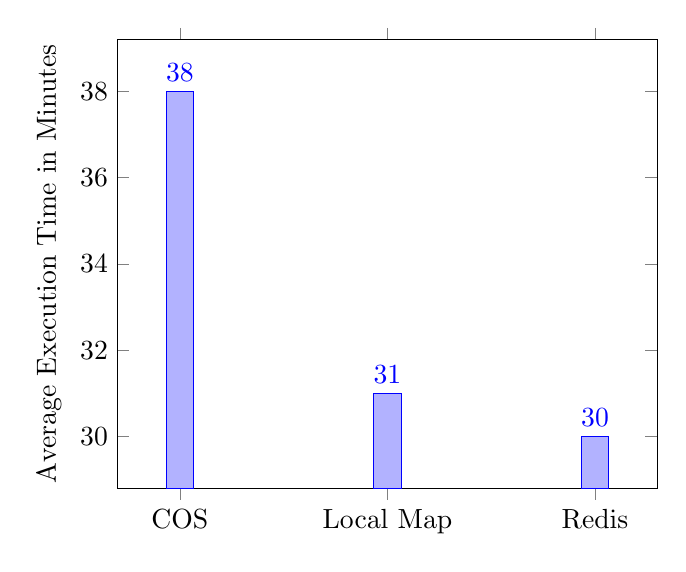
\begin{tikzpicture}
\begin{axis}[
    ybar,
    enlargelimits=0.15,
    legend style={at={(0.5,-0.15)},
      anchor=north,legend columns=-1},
    ylabel=Average Execution Time in Minutes,
    symbolic x coords={COS,Local Map,Redis},
    xtick=data,
    nodes near coords,
    nodes near coords align={vertical},
    ]
\addplot coordinates {(COS,38) (Local Map,31) (Redis,30)};
\end{axis}
\end{tikzpicture}
\caption{\textit{\textbf{Serverless Prototypes Average Execution Time}}}
\end{figure}


\vspace{2mm}
\subsubsection{Cost Analysis}
As we can observe from figure number 3, COS Prototype is the most expensive implementation followed by Work Queue, then by Local Map Prototype, and the last is the Redis Prototype. The reason why COS Prototype is the most expensive is the average function execution time and the IBM Cloud Functions price scheme. In this case the operations against IBM COS Buckets do not have any influence in the final price. Indeed, we depreciate the COS operations in this analysis, because the magnitude order of the price is approximately 0.5 American dollars for GET operations and 1.6 American dollars for PUT operations for each prototype.

On the other hand, the Redis prototype is cheaper due to the fact that the average execution time of the serverless functions is less than the average execution time of the remaining prototypes. This is due to the IBM functions pricing schema is calculated per execution second per GB of memory  assigned. Therefore, if we estimate the total price of executing all functions for each prototype with the help of the IBM Functions Cost Estimator\cite{ibmCostEstimator}, we observe that Redis Prototype holds the lowest total cost in terms of functions executions. Thus, despite this prototype having an extra cost related with the requirement to configure an extra virtual server to host the Redis database, it maintains the cheaper total cost by holding the functions lower average execution time.


\pgfplotsset{compat=1.14}
\begin{figure}[t]
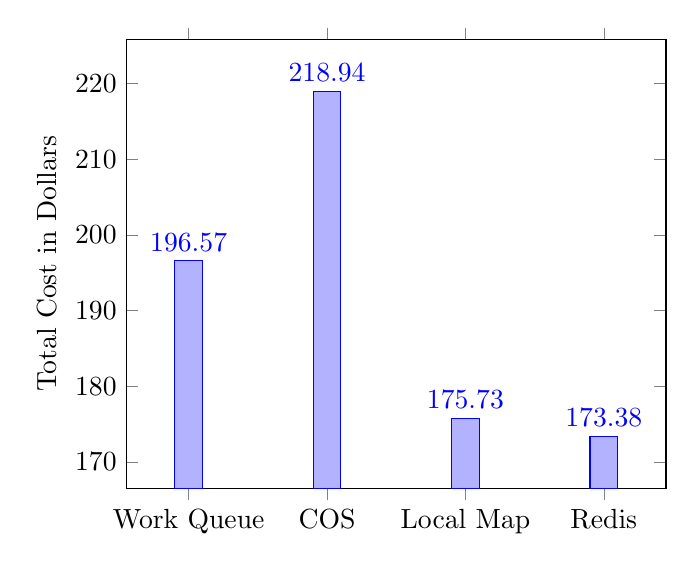
\begin{tikzpicture}
\begin{axis}[
    ybar,
    enlargelimits=0.15,
    legend style={at={(0.5,-0.15)},
      anchor=north,legend columns=-1},
    ylabel=Total Cost in Dollars,
    symbolic x coords={Work Queue, COS,Local Map,Redis},
    xtick=data,
    nodes near coords,
    nodes near coords align={vertical},
    ]
\addplot coordinates {(Work Queue,196.57) (COS,218.94) (Local Map,175.73) (Redis,173.38)};
\end{axis}
\end{tikzpicture}
\caption{\textit{\textbf{Serverless vs Work Queue Cost Comparison}}}
\end{figure}



\subsubsection{Scalability Analysis}
We can figure out that our serverless prototypes scale transparently, whereas the Work Queue implementation does not. In Work Queue, the number of parallel tasks supported by an application is measured by the number of workers available in the cluster. At the same time, each worker must be explicitly started by the application users and each requires a vCPU core to function properly. Therefore, it means that if we want to increase the parallelism degree supported by our application, we will require to start new workers, which could also mean providing more hardware resources to increment the number of vCPU cores available in the cluster. As we can observe, that was exactly what happened in our experiments. With the growth of the number of replicas configured in the Replica Exchange through the iterations of the experiment, it was mandatory to add more virtual servers to satisfy the number of  vCPU cores required to execute the count of workers needed.

On the other hand, we observe that serverless prototypes scale transparently according to application load. With our prototypes, when the number of Replica Exchange replicas grows, the number of functions invoked grows dynamically without providing extra configurations or hardware. In the following code snippet we observe how IBM-PyWren manages these invocations:

\lstset{style=mystyle}
\begin{lstlisting}[language=Python]
pw = pywren.ibm_cf_executor(runtime='cactusone/pywren-protomol:3.6.14', runtime_memory=2048)
pw.map(serverless_task_process, task_list_iterdata)

\end{lstlisting}

Through the executor object, we define the memory assigned to each serverless function. In this case, we assign 2048 MB that ensures one vCPU core for each function executed. Furthermore, with the map function, IBM-PyWren invokes the serverless functions execution. Whereas the first parameter refers to the name of the function to be executed as serverless, the second parameter is a list whose size define the number of functions to be executed in parallel. Additionally, each position in the list contains the value assigned as an input argument for a launched function. If our functions require two or more parameters, it is possible to build a list of dictionaries using as dictionary keys, the name of the arguments defined in the function.

\section{Conclusions}
As we observed throughout this paper, serverless prototypes reduce the total execution time of the Replica Exchange around a forty percent in comparison with Work Queue. This is because our prototypes avoid the data exchange between the master and the workers that occurs in Work Queue. Instead of this, our prototypes make use of desegregated key-value storages to save and share the required data. Also, from the serverless prototypes perspective, the COS Prototype is the slowest. This is due to the fact that cloud object storages are not prepared to support fine-grained operations. In addition to this, Redis and Local Dictionary prototypes make use of in-memory storages and they have similar execution times because the network latency is negligible when the database instance and the functions that access it share the same availability zone.

From the scalability perspective, serverless prototypes have been transparently scaled. As we observed in the experiment, regardless of the number of replicas configured in Replica Exchange, our prototypes have managed the load correctly without explicitly configuring additional resources. On the other hand, with Work Queue is mandatory to add additional VMs and workers according to the growth of replicas configured in the iterations of the experiment.

From the cost standpoint, we have found that getting a faster and transparently scalable solution does not mean a more expensive solution. In fact, it could be cheaper if we take the total cost of Redis and Local Dictionary prototypes.

In terms of related future work, the access transparency principle emerges as the next step in the movement of Proteomic applications to cloud platforms. Following this principle, the applications would be able to manage cloud resources as local resources. As a consequence, the applications will be agnostic and they will be available to be deployed in multiple clouds without affecting the source code of them.


\nocite{GarcaLpez2020ServerlessEG}
\nocite{wqFolding}

\label{sec:conclusions}


\medskip
\bibliographystyle{ACM-Reference-Format}
\bibliography{main}
\end{document}
%%
%% The next two lines define the bibliography style to be used, and
%% the bibliography file.


\endinput
